\section{Socket Programming}
\subsection{Socket 이란?}
    소켓(Socket)은 컴퓨터 네트워크를 경유하는 프로세스 간 통신의 종착점이다. 인터넷 프로토콜(IP, Internet Protocol)에 기반한 네트워크 소켓을 인터넷 소켓이라고 한다. 모든 네트워크 응용 프로그램은 통신을 위한 소켓을 생성하고, 이 소켓을 통해 데이터를 송수신한다. 두 호스트를 연결한 소캣은 역할에 따라 서버 소켓과 클라이언트 소켓으로 구분된다. \\
    \vspace{-4mm}
    \begin{figure}[!h]\centering
		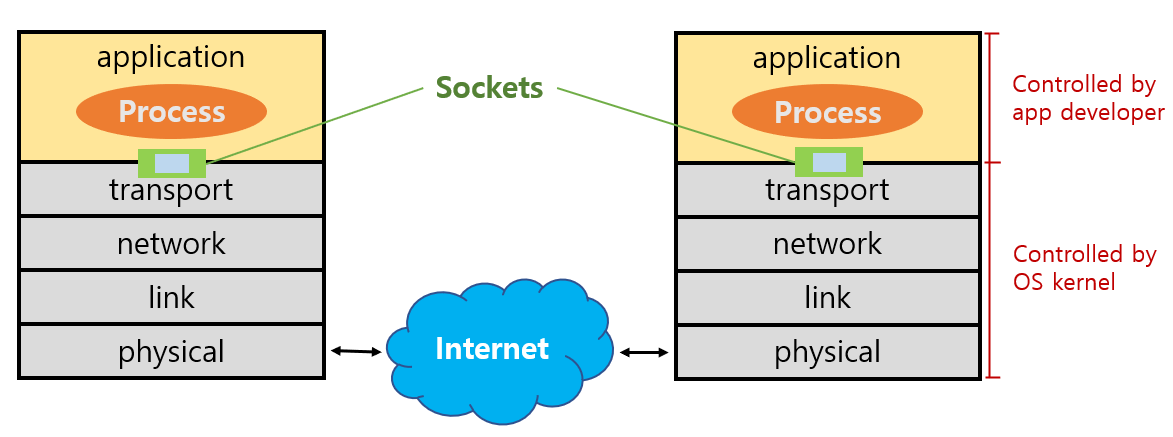
\includegraphics[width=.65\textwidth]{image/week07/1-1.png}
		\caption{\small Socket}
		\vspace{-10pt}
    \end{figure}
    
\subsection{소켓통신을 위해 필요한 것들}    
    소켓은 프로토콜, IP 주소, Port 번호로 정의된다. \\
    
    \textbf{프로토콜:} 컴퓨터 내부에서, 또는 컴퓨터 사이에서 데이터의 교환 방식을 정의하는 규칙 체계로, 소켓 통신의 경우 전송 계층(Transport Layer) 위의 TCP 또는 UDP가 쓰인다. \\
    \textbf{IP 주소:} 호스트(컴퓨터, 스마트 폰 등의 단말기)들을 식별할 수 있는 고유한 주소 \\
    \textbf{Port 번호:} 호스트 내의 프로세스들을 식별할 수 있는 번호 \\
    
\subsection{TCP/IP 와 UDP/IP}    
    TCP와 UDP는 클라이언트와 서버 간의 통신 채널을 제공하는 4계층(Transport Layer)의 프로토콜이다. TCP/IP와 UDP/IP는 3계층의 IP(Internet Protocol)와 4계층의 TCP와 UDP를 합쳐 통신을 하는 프로토콜으로, 현재 인터넷 통신의 일반적인 통신 모델이다. IP는 데이터를 알맞은 IP 주소를 갖는 호스트로 전달하고, TCP와 UDP는 데이터를 알맞은 Port 번호를 갖는 프로세스로 전달한다. \\
    \vspace{-4mm}
    \begin{figure}[!h]\centering
		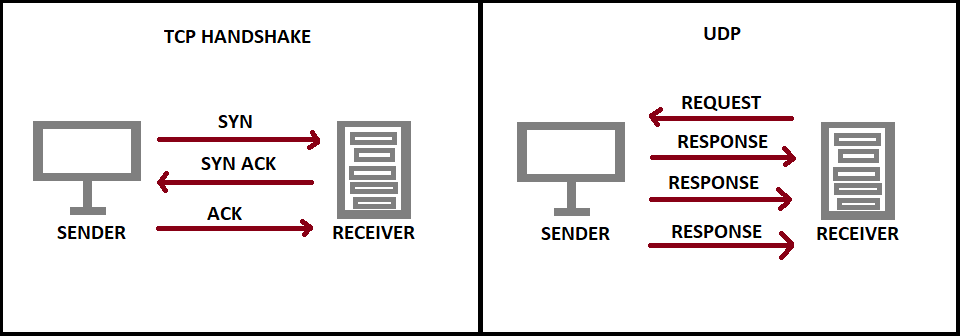
\includegraphics[width=.65\textwidth]{image/week07/1-2.png}
		\caption{\small TCP and UDP}
		\vspace{-10pt}
    \end{figure}
    
    \subsubsection*{TCP(Transmission Control Protocol)}
    TCP는 신뢰성 있는 데이터 전송을 지원하는 연결 지향형 프로토콜이다. 3-way handshaking이라는 과정을 통해 연결하고 4-way handshaking으로 통신을 끊는 연결형 서비스로 가상 회선 방식을 제공한다. \\
    네트워크에서 신뢰성 있는 데이터 전송(Reliable Network)를 보장하기 위해서 다음 4개의 문제를 해결해야 한다. \\
    \begin{enumerate}
        \item 손실: Packet이 손실될 수 있다.
        \item 순서 바뀜: Packet의 순서가 바뀔 수 있다.
        \item Congestion: 네트워크가 혼잡할 수 있다.
        \item Overload: Receiver가 overload 될 수 있다.
    \end{enumerate}
    TCP 프로토콜은 데이터를 여러 packet으로 나누고, 그 packet을 보낼 때 순서에 맞게 Seq(Sequence number)를 붙이고, 응답으로 ACK(Acknowledgement number)를 받는 통신 과정을 통해 packet의 손실을 방지하고 순서를 보장한다. 또, 송신 측의 데이터 전송량을 수신측에 따라 조절하는 흐름 제어(Flow Control)와 네트워크 상황에 따라 송신 측의 데이터 전송량을 조절하는 혼잡 제어(Congestion Control)를 지원하여 신뢰성 있는 데이터 전송을 보장한다. \\
    TCP는 신뢰성 있는 데이터 전송을 보장하는 대신 UDP에 비해 느리다. 따라서 빠른 데이터 통신보다 신뢰성이 더 중요한 HTTP, Telnet, FTP, POP 등의 상위 프로토콜을 전달하는데 쓰인다. web 페이지, 메일의 송수신, 파일 전송, 공유에 적절하다. \\
    
    \subsubsection*{UDP(User Datagram Protocol)}
    UDP는 데이터를 송수신할때 TCP처럼 정보를 보낸다는 신호나 받는다는 신호를 받는 과정을 거치지 않고 서로 일방적으로 데이터를 전송하는 비연결형 통신 프로토콜이다. TCP와 다르게 연결 설정이 없고 혼잡 제어를 하지 않아 신뢰성 있는 데이터 전송을 보장하지 못하지만 TCP보다 전송 속도가 빠르다. 따라서 어느 정도의 packet 손실이 용인되지만 속도에 민감한 DNS, NTP, DHCP, SNMP 등의 상위 프로토콜을 전달하는데 쓰인다. 음성통화, Video 스트리밍, 멀티캐스트 통신, 브로드캐스트 통신, 소량의 데이터 통신에 적절하다. \\

\newpage    
\subsection{소켓프로그래밍 진행과정}    
    인터넷 소켓은 TCP/IP을 이용하는 경우와 UDP/IP을 이용하는 경우, 두 개의 타입으로 분류할 수 있다. \\
    
    \subsubsection*{TCP/IP Socket Programming}
    \vspace{-4mm}
    \begin{figure}[!h]\centering
		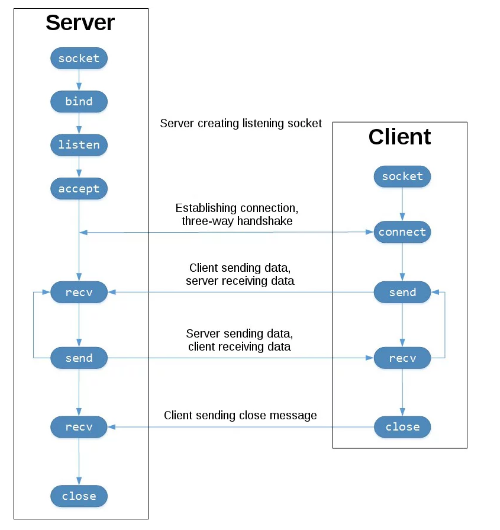
\includegraphics[width=.65\textwidth]{image/week07/1-3.png}
		\caption{\small TCP/IP Socket Programming}
		\vspace{-10pt}
    \end{figure}
    TCP/IP의 소켓프로그래밍 진행과정은 다음과 같다. \\
    \textbf{Server}
    \begin{enumerate}
        \item Socket: Server 소켓 생성
        \item Bind: Server의 IP 주소와 Port 번호 설정
        \item Listen: Client로부터 연결 요청이 있는지 수신 대기
        \item Accept: Client의 연결 요청을 수락하는 실질적 소켓 연결 단계
    \end{enumerate}
    
    \textbf{Client}
    \begin{enumerate}
        \item Socket: Client 소켓 생성
        \item Connect: IP 주소와 Port 번호로 식별되는 Server에게 연결 요청
    \end{enumerate}
    이후 Send와 Receive 단계를 반복하며 Client는 데이터를 요청하고 Server는 요청받은 데이터를 보낸다. 데이터 송수신을 마치고 Client가 Server에게 Close 메시지를 보냄으로써 연결을 끊는다. \\
    
\newpage  
    \subsubsection*{UDP/IP Socket Programming}
    \vspace{-4mm}
    \begin{figure}[!h]\centering
		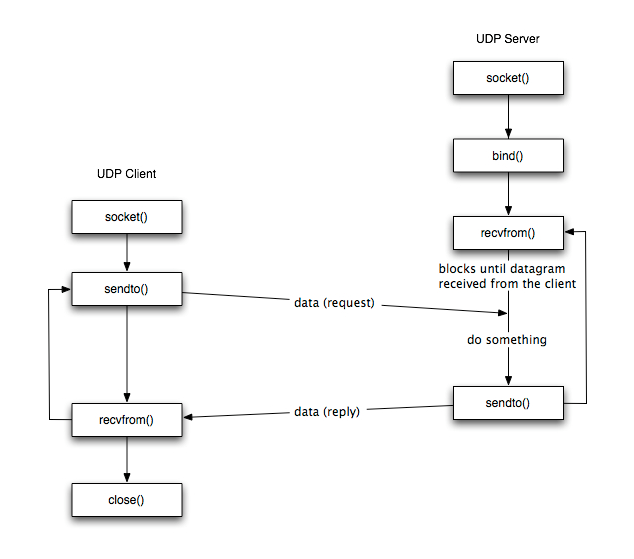
\includegraphics[width=.65\textwidth]{image/week07/1-4.png}
		\caption{\small UDP/IP Socket Programming}
		\vspace{-10pt}
    \end{figure}
    UDP/IP 소켓프로그래밍의 경우, TCP와 유사하나 Server의 Listen과 Accept, Client의 Connect에 해당하는 연결 과정 없이 소켓을 생성한 후 데이터를 바로 전송한다. \\
    
\subsection{Round trip time (RTT) 이란?}    
    RTT는 패킷망(인터넷)에서 데이터 패킷이 송신지에서 목적지까지 패킷이 왕복하는데 걸리는 시간이다. 네트워크 연결의 속도와 안정성을 진단할 때 사용된다. RTT에 영향을 주는 요소에는 거리, 전송 매체, 네트워크 홉 수, 네트워크 트래픽 수준, 서버 응답 시간 등이 있다. \\
% \newpage